\documentclass[a4paper,12pt]{extarticle}

% Даёшь нормальную кодировку!
\usepackage[utf8]{inputenc}

% Тщетные попытки включить Times New Roman
\usepackage[T1]{fontenc}
%\font\ttftimes times at12pt
%\usepackage{mathptmx}
%\usepackage{txfonts}

% Вставка картинок из директории images
\usepackage[dvips]{graphicx}
\graphicspath{{images/}}
\usepackage[usenames, dvipsnames]{color} % цвет

% Набор математических пакетов
\usepackage{amsmath}
\usepackage{amsfonts}
\usepackage{amssymb}
\usepackage{amsthm}
\usepackage{multirow}
\usepackage{tikz}
%\usepackage{longtable}
\usepackage{pdfpages}

\usepackage{cmap} % поиск русских слов и вообще поддержка русского
\usepackage[english, russian]{babel}

\usepackage{listings}
\usepackage{verbatim}
\renewcommand{\lstlistingname}{Листинг}

\usepackage{statmodtitle}
\usepackage{indentfirst} % абзацный отступ после заголовка
\setcounter{tocdepth}{2} % Не отображать subsubsection и ниже в содержании
\bibliographystyle{unsrt}

% Поля и полуторный межстрочный интервал
\usepackage{setspace}
\usepackage[left=30mm,right=15mm,top=20mm,bottom=20mm]{geometry}
\onehalfspacing
% Начинать каждый раздел с новой страницы
\let\stdsection\section
\renewcommand\section{
    \newpage
    \stdsection
}

\setcounter{page}{1} % Резервируем первую страницу для титульного листа
\renewcommand{\arraystretch}{1.5} % Изменяем высоту строк таблицы

\lstset{ %
  backgroundcolor=\color{white},   % choose the background color; you must add \usepackage{color} or \usepackage{xcolor}
  basicstyle=\footnotesize,        % the size of the fonts that are used for the code
  breakatwhitespace=false,         % sets if automatic breaks should only happen at whitespace
  breaklines=true,                 % sets automatic line breaking
  captionpos=t,                    % sets the caption-position to bottom
  commentstyle=\color{green},    % comment style
  deletekeywords={...},            % if you want to delete keywords from the given language
  escapeinside={\%*}{*)},          % if you want to add LaTeX within your code
  extendedchars=true,              % lets you use non-ASCII characters; for 8-bits encodings only, does not work with UTF-8
%  frame=single,                    % adds a frame around the code
  keepspaces=true,                 % keeps spaces in text, useful for keeping indentation of code (possibly needs columns=flexible)
  keywordstyle=\color{blue},       % keyword style
  language=C++,                 % the language of the code
  morekeywords={*,...},            % if you want to add more keywords to the set
  numbers=left,                    % where to put the line-numbers; possible values are (none, left, right)
%  numbersep=5pt,                   % how far the line-numbers are from the code
%  numberstyle=\tiny\color{mygray}, % the style that is used for the line-numbers
  rulecolor=\color{black},         % if not set, the frame-color may be changed on line-breaks within not-black text (e.g. comments (green here))
  showspaces=false,                % show spaces everywhere adding particular underscores; it overrides 'showstringspaces'
  showstringspaces=false,          % underline spaces within strings only
  showtabs=false,                  % show tabs within strings adding particular underscores
  stepnumber=1,                    % the step between two line-numbers. If it's 1, each line will be numbered
  stringstyle=\color{mymauve},     % string literal style
  tabsize=4,                       % sets default tabsize to 2 spaces
  title=\lstname,                   % show the filename of files included with \lstinputlisting; also try caption instead of title
  basicstyle=\footnotesize\ttfamily,
  keywordstyle=\bfseries\color{green!40!black},
  commentstyle=\itshape\color{purple!40!black},
  identifierstyle=\color{blue},
  stringstyle=\color{orange}
}

% всё тлен и безысходность

\date{2012-06-19}
\title{Разработка интерактивной системы визуализации данных в физических моделях}
\author{Зайцев Вадим, ФИТ НГУ, 9204}

\renewcommand{\rmdefault}{ftm}



\begin{document}


\includepdf{tlb.pdf}

\tableofcontents

\section*{Введение}
\addcontentsline{toc}{section}{Введение} % Добавляем в содержание раздел без номера
\label{sec:intro}

Благодаря быстрому развитию вычислительной техники, моделирование стало одним из основных способов исследования физических процессов, наряду с экспериментом и теорией. Во многих случаях изучение явления с использованием модели менее затратное в сравнении с проведением эксперимента, а иногда эксперимент невозможно провести в принципе.

Один из основных видов моделирования --- имитационное моделирование. Для него характерно описание моделируемого объекта в виде программы, имитирующей его работу. В рамках имитационного моделирования возможно построение моделей для широкого спектра физических явлений с такой сложностью протекающих в них процессов, которая не позволяет описать их в аналитической форме. 

Для описания физических процессов широкое распространение получил класс имитационных моделей на основе алгоритмов с мелкозернистым параллелизмом (далее --- МЗП-модели). Мелкозернистый параллелизм (МЗП), наряду с крупноблочным, является одним из двух базовых видов параллелизма. Его отличительная черта --- большое число простых параллельно выполняемых преобразований данных, распределенных в пространстве. К широко известным классам алгоритмов с мелкозернистым параллелизмом относятся классический клеточный автомат (КА) и его расширения (КА с окрестностью Марголуса~\cite{toff}, асинхронный КА, вероятностный КА), сеть КА, клеточно-нейронная сеть, дискретная динамическая сеть, системы Линденмайера. Алгоритмы и структуры с МЗП используются для моделирования физических, химических, биологических и социальных процессов, разнообразных вычислительных устройств (ассоциативный процессор, систолическая структура, однородная среда, универсальная вычислительная среда, конвейеры арифметических устройств)~\cite{il}.

\textbf{Цель работы} --- обеспечить исследователя МЗП моделей физических процессов инструментом для построения и отладки таких моделей и визуализации данных в них. Хотя система должна обладать достаточной универсальностью и быть пригодной для широкого спектра таких моделей, в первую очередь рассматривается визуализация данных для клеточно-автоматных моделей газов.

\textbf{Актуальность}. Рассматриваемый класс моделей характерен сложностью происходящих в них преобразований данных и большим объёмом данных. Под большим объёмом данных подразумевается, что он существенно превосходит размеры оперативной памяти отдельного узла. Сложность преобразований данных в моделях означает необходимость:
\begin{enumerate}
    \item отладки модели в процессе её создания;
    \item создания режимов визуализации, позволяющих исследователю увидеть как точную количественную картину некоторого фрагмента состояния модели, так и качественную картину протекающих в модели процессов.
\end{enumerate}

Если исследователь выбирает путь построения собственной программы визуализации, он неизбежно сталкивается с необходимостью реализации системных функций, сложность которых значительно выше, чем само описание модели. Таким образом, для эффективной работы исследователя необходим инструмент для построения, отладки и исследования моделей.

В первой главе сформулированы требования, предъявляемые к разрабатываемой системе. Главными из них являются адекватность системы проблемной области, открытость архитектуры и возможность работы с большими объёмами данных.

Во второй главе приводится обзор существующих систем, имеющих средства визуализации моделей. Проведён анализ на предмет их соответствия полученным требованиям, который показал, что ни одна из рассмотренный систем не удовлетворяет им в полной мере.

В третьей главе дано описание архитектуры системы. В частности, рассматриваются методы, используемые при проектировании системы, и её модульная структура. Приведено описание реализованной подсистемы визуализации.




\section{Формирование требований}
\label{sec:requirements}

Назначение системы --- визуализация данных в МЗП-моделях физических процессов.  Наиболее существенное требование, требование адекватности системы проблемной области, заключается в создании удобного инструмента, содержащего все необходимые исследователю функции для изучения широкого спектра таких моделей.

Моделирования физических явлений с помощью МЗП-моделей --- динамично развивающаяся область, в которой постоянно возникают новые классы моделей. Для того, чтобы система могла применяться для них, она должна иметь открытую архитектуру, позволяя пополнять свой набор функций не только разработчикам, но и пользователям системы. 

Для МЗП-моделей физических явлений характерно то, что адекватность результатов достигается только при очень больших размерах объектов: во-первых, не все явления могут быть заметны на моделях маленького размера, во-вторых, за счёт увеличения размера объекта достигается более точный результат.

Таким образом, основными требованиями, предъявляемыми к системе, являются:
\begin{itemize}
    \item адекватность проблемной области;
    \item открытая архитектура;
    \item обработка больших объёмов данных;
\end{itemize}

Далее будет подробно рассмотрено, что включает в себя каждое из приведённых требований.

\begin{subsection}{Адекватность проблемной области}
    \label{sec:requirements-adequacy}

    Адекватность системы предметной области означает удовлетворение системой требованиям, которые предъявляет к ней исследователь в данной предметной области: так как система создаётся для работы с МЗП-моделями, то она должна реализовывать необходимые функции, требующиеся при изучении данной области, а именно:
    \begin{itemize}
        \item построение моделей;
        \item управление проектами;
        \item исполнение модели;
        \item изучение модели;
        \item отладка модели.
    \end{itemize}

    \begin{subsubsection}{Построение моделей}
        С точки зрения системы модель определяется правилами, задающими поведение моделируемых объектов, параметрами данных объектов (например, для моделей клеточных автоматов это будут правила, по которым которым осуществляются переходы в ячейках, массы частиц покоя и количество движущихся частиц) и объектом данных, над которым производятся вычисления. Объектом данных является структура, хранящая в себе состояние моделируемого объекта. Такая структура может быть как и многомерным массивов так и нерегулярной структурой данных.
        
        Исследователю необходимо иметь возможность формировать и корректировать параметры модели и создавать и редактировать объекты данных. Для работы с моделью удобно наличие визуальной среды: графический пользовательский интерфейс упрощает работу с множеством параметров модели и с большими объектами данных.
        
        Свойства модели могут быть представлены значениями произвольных типов (число, строка, массив значений и т. п.). Объект данных может быть как небольшого (обычно такие объекты используются при отладке модели), так и огромного размера. И в том, и в другом случае бывает необходимость редактировать значения как отдельных ячеек, так и их групп.
    \end{subsubsection}
        
    \begin{subsubsection}{Управление проектами}
        В процессе исследования возникает необходимость скорректировать параметры изучаемой модели, посмотреть на изменение поведения, сравнить данную модель с исходной по каким-либо характеристикам. В таких случаях удобно объединять две и более модели в один проект с возможностью сохранения и загрузки проекта. 
        
        Проект можно определить как группу логически связанных между собой моделей, при этом определение модели расширяется, в проекте с моделью ассоциируются пользовательские настройки (например, сохранение настроек режимов визуализации для данной модели). В проект можно добавлять новые модели, удалять из него старые. Основными функциями проекта являются сохранение открытого проекта с возможностью последующей загрузки.
    \end{subsubsection}
        
    \begin{subsubsection}{Исполнение модели} 
        Одной из основных функций является счёт модели, который включает в себя передачу параметров модели и объекта данных на вычислитель, запуск модели на фиксированное число итераций, ожидание завершения счёта и последующее получение результирующих данных с вычислителя.
        
        Под вычислителем понимается устройство, на котором происходит исполнение модели. Вычислителем может выступать такое устройство локального или удалённого компьютера, как центральный или графический процессор. Вычислитель при этом необязательно является однопроцессорной машиной: в его роли могут так же выступать мультипроцессорные системы, системы с распределённой памятью, кластеры и ГРИД-системы.
    \end{subsubsection}
        
    \begin{subsubsection}{Изучение модели}
        При работе с моделями пользователь системы нуждается в  визуализации объекта данных модели не только на микроуровне, но и на макроуровне, позволяющем увидеть качественную картину. Например, иметь возможность выделить из всего объекта данных какую-либо конкретную характеристику. Так же пользователю необходимо дать возможность быть не только пассивным наблюдателем, но и активно влиять на процесс моделирования, т. е. требуется обеспечить интерактивность системы.
        
        Качественная картина может быть предоставлена за счёт поддержки различных режимов визуализации (режимом визуализации является функция, отображающая объект данных в изображение, которое впоследствии может быть выведено на экран монитора): например, это может быть режим осреднённых плотностей или профиль волны для исследования её поведения. На макроуровне полезными могут быть не только режимы, визуализирующие какую-либо конкретную численную характеристику (плотность частиц, направление потоков), но и режимы, формирующие целостную картину. Например, трёхмерный режим с возможностью масштабирования и вращения для просмотра объекта данных с разных ракурсов.
    \end{subsubsection}
        
    \begin{subsubsection}{Отладка модели}
        При построении больших и сложных моделей могут возникать ошибки в их описании. В таких случаях модель приходится отлаживать: использовать какие-либо средства с целью выявления допущенных ошибок. Система в свою очередь должна помочь исследователю, предоставив такие средства.
        
        В процессе отладки востребован не только запуск счёта модели на фиксированное, большое количество итераций, но и запуск модели в \textit{режиме} пошагового исполнения: формирование модели и отправка её на вычислитель, запуск на небольшое количество шагов, получение промежуточных данных с возможностью продолжить вычисления с того момента, где они были приостановлены. Пошаговое исполнение позволяет детальнее изучить поведение модели.
        
        При отладке востребована возможность модификации текущего объекта данных, передача изменений на вычислитель и продолжение счёта.
    \end{subsubsection}

\end{subsection}

\begin{subsection}{Открытая архитектура}
    \label{sec:requirements-open}
    
    Открытость архитектуры облегчает сопровождение системы и её адаптацию к изменяющимся требованиям.

    Свойство открытости включает в себя \cite{filinov-os}:
    \begin{itemize}
        \item расширяемость;
        \item переносимость;
        \item интероперабельность;
        \item дружественность интерфейса.
    \end{itemize}

    \begin{subsubsection}{Расширяемость}
        Потенциальные пользователи системы уже имеют набор активно используемых программ, устоявшиеся форматы данные в этим форматах. Требуется создание универсального инструмента, способного поддерживать существующие форматы и адаптироваться в будущем под новые требования. Поскольку не представляется возможным реализовать поддержку всех используемых форматов данных, обеспечить совместимость со всеми системами моделирования, то вместо этого необходимо предоставить пользователям механизм включения собственных реализаций работы с форматами данных, поддержки новых классов моделей, ранее не предусмотренных системой.
        
        Направлениями для расширения системы являются:
        \begin{itemize}
            \item форматы данных;
            \item режимы визуализации;
            \item поддержка графических библиотек;
            \item коммуникация с подсистемой моделирования.
        \end{itemize}
        
        Формат данных определяет правила кодирования информации. Существует огромное множество различных форматов данных, постоянно появляются новые, потому требуется механизмы, с помощью которых можно либо добавить в систему поддержку нового формата, либо добавить возможность конвертации нового формата в один из тех, с которыми система уже умеет работать.
        
        В процессе исследования требуется смотреть на различного рода характеристики и невозможно заранее предугадать, какого рода данные предстоит визуализировать. Поддержка добавления новых режимов со стороны системы даёт исследователю инструменты для визуализирования любой характеристику, тем самым решая данную проблему.
        
        Помимо поддержки новых форматов данных и новых режимов визуализации, так же должна быть возможность встраивать поддержку новых графических библиотек (например, рисование трёхмерных изображений под ОС Windows делать не с помощью OpenGL, а с использованием библиотеки Direct3D). 
        
        Ещё одним направлением расширения системы является добавление поддержки альтернативных способов коммуникации с вычислителем: например, когда в качестве вычислителя вместо центрального процессора выступает видеокарта, то обмен данными уже невозможно организовать через общую память и потребуется реализовать передачу данных между оперативной памятью компьютера (к которой система визуализации имеет прямой доступ) и памятью графического ускорителя.
        
        Всё это требует от системы масштабируемости по архитектуре: возможность вносить изменения, связанные с добавлением нового функционала, при этом минимизируя влияние (т. е. либо не требуя модификации, либо модификация существующей реализации должна быть незначительной) на другие, уже существующие компоненты системы.
    \end{subsubsection}
        
    \begin{subsubsection}{Переносимость}
        С течением времени архитектуры процессоров и операционные системы меняются. Создание системы, привязанной к одной конкретной платформе, может в будущем потребовать значительных усилий для портирования системы под другую платформу или вовсе привести к прекращению поддержки системы, когда используемая платформа устареет.
        
        Второй проблемой при разработке платформозависимой системы является проблема взаимодействия с приложениями, привязанными к другим платформам. Это потребует от пользователей либо портировать их приложения на используемую системой платформу, либо отказаться от использования системы.
        
        Таким образом, от системы требуется свойство переносимости --- отсутствие  зависимостей модулей системы от конкретной платформы. В системе допускается привязка отдельных реализаций некоторых компонентов к определённым платформам, но в целом она должна оставаться платформонезависимой.
        
        Переносимость должна быть обеспечена на уровне исходного кода (код приложения не должен использовать платформозависимые библиотеки или функции или же функциональность, достигаемая с использованием данных библиотек, должна быть реализована для каждой платформы) и на уровне данных (работа с созданными проектами и моделями на одной платформе должна быть возможна и на других платформах) \cite{ieee}.
    \end{subsubsection}
        
    \begin{subsubsection}{Интероперабельность}
        Интероперабельность для подсистемы визуализации способность системы взаимодействовать с окружением, в котором она запущена. Для подсистемы визуализации это, в первую очередь, способность взаимодействовать с подсистемой моделирования.
        
        Взаимодействие основывается на использовании общих форматов хранения данных, интерфейсов для взаимодействия на локальных системах или протоколов для взаимодействия в распределённых средах. Благодаря интероперабельности система визуализации может использоваться как звено в цепи обработки информации, получая входные данные от подсистемы моделирования, отрисовывая полученные данные и передавая созданные изображения другим приложениям для последующей обработки.
    \end{subsubsection}
        
    \begin{subsubsection}{Дружественность интерфейса}
        Интерфейс системы можно разделить на интерфейс пользователя и программный интерфейс \cite{ieee}.
        
        Дружественность пользовательского интерфейса заключается в наличии интуитивно-понятного и комфортного взаимодействия системы с пользователем. Требование является необходим для любой отчуждаемой от разработчиков программы, в которой присутствует функция взаимодействия с пользователем.
        
        Дружественность программного интерфейса относится к разработчикам системы (как и к тем, кто изначально разрабатывает систему, так и к пользователям, которые будут расширять систему за счёт встраивания своих модулей) и означает упрощение разработки системы: интерфейсы, дающие возможности для расширения системы, должны требовать реализацию только минимального необходимого набора методов.
    \end{subsubsection}

\end{subsection}

\subsection{Обработка больших объёмов данных}

Требование к поддержки больших объёмов данных обусловлено особенностью моделей физических явлений:
\begin{enumerate}
    \item Многие явление могут быть незаметны на моделях маленького размера (например, вихри --- они проявляются только на объектах больших размеров).
    
    \item Как правило, при увеличении размера объекта данных, при более сильном дроблении, качество моделирования повышается и результат получается более точным.
\end{enumerate}

Под возможностью обработки больших объёмов данных понимается способность системы визуализировать объекты данных, размер которых превышают размер оперативной памяти компьютера.


\begin{section}{Обзор существующих систем}

На сегодняшний день существует немало средств моделирования и визуализации, потому следующим этапом после формирования требований был обзор уже существующих систем.

Далее приведён обзор нескольких, наиболее подходящих под предъявляемые требования, систем. Полный список обозреваемых систем и их соответствие требованиям приведён в Приложении А. 

\begin{subsection}{Mirek's Celebration}
    Система моделирования 1D и 2D клеточно-автоматных моделей. Имеет богатые возможности по редактированию объектов данных и инструменты для проведения анализа
    Так же присутствует подробная документация.

    \begin{table}[h]
        \caption{Соответствие требованиям системы Mirek's Celebration}
        \label{tabular:mirekscell}
        \begin{center}
            \begin{tabular}{|p{0.35\linewidth}|p{0.05\linewidth}|p{0.5\linewidth}|} \hline
                Адекватность пред. области & + & Система ориентирована на КА модели. \\ \hline
                Расширяемость              & $\pm$ & Есть возможности встраивания DLL, однако, возможности расширения ограничены. \\ \hline
                Интероперабельность        & + & Поддержка многих существующих форматов файлов КА.\\ \hline
                Платформонезависимость     & -- & Прилоежние написано под платформу Win32. \\ \hline
                Дружественный интерфейс    & + & Удобный, интуитивно-понятный пользовательский интерфейс. \\ \hline
                Большие объёмы данных      & -- & Моделирование происходит на центральном процессоре локальной машины. \\ \hline
            \end{tabular}
        \end{center}
    \end{table}
\end{subsection}

\begin{subsection}{WinALT}
    Система визуального проектирования и отладки
    Система моделирования широкого спектра МЗП-моделей, в первую очередь алгоритмов и структур.
    \newpage
    
    \begin{table}[h]
        \caption{Соответствие требованиям системы WinALT}
        \label{tabular:winalt}
        \begin{center}
            \begin{tabular}{|p{0.35\linewidth}|p{0.05\linewidth}|p{0.5\linewidth}|} \hline
                Адекватность пред. области & + & \\ \hline
                Расширяемость              & + & \\ \hline
                Интероперабельность        & + & \\ \hline
                Платформонезависимость     & + & Графическая среда платформозависима и привязана к ОС Windows. Ядро и консольная версия платформозависимы. \\ \hline
                Дружественный интерфейс    & + & \\ \hline
                Большие объёмы данных      & -- & \\ \hline            
            \end{tabular}
        \end{center}
    \end{table}
\end{subsection}

\begin{subsection}{Ansys Fluent}
    Система моделирования широкого спектра физических процессов, в том числе и процессов газовой динамики, обладает богатыми возможностями моделирования и визуализации.

    \begin{table}[h]
        \caption{Соответствие требованиям системы Ansys Fluent}
        \label{tabular:ansysfluent}
        \begin{center}
            \begin{tabular}{|p{0.35\linewidth}|p{0.05\linewidth}|p{0.5\linewidth}|} \hline
                Адекватность пред. области & -- & Дифференциальные уравнения решаются классическими методами. \\ \hline
                Расширяемость              & + & Есть возможность встраивания пользовательских функций. \\ \hline
                Интероперабельность        & + & \\ \hline
                Платформонезависимость     & + & \\ \hline
                Дружественный интерфейс    & + & \\ \hline
                Большие объёмы данных      & + & Есть возожность запуска счёта на кластерах. \\ \hline
            \end{tabular}
        \end{center}
    \end{table}
\end{subsection}

\newpage
\subsection{Выводы}

Таким образом, ни одна из рассмотренных систем в полной мере не удовлетворяет всем предъявленным к ней требованиям и было решено создать собственную реализацию системы визуализации. На рисунке~\ref{ris:systems-simulus} предствлены все требования в виде окруностей, в пересечение всех трёх которых не попадает ни одна система, хотя существуют системы, удовлетворяющие одному-двум свойствам.

\begin{figure}[h]
    \center{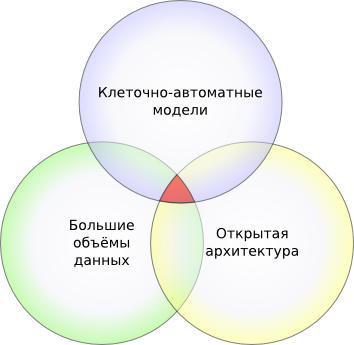
\includegraphics[width=.5\linewidth]{systems-simulus}}
    \caption{Существующие системы визуализации}
    \label{ris:systems-simulus}
\end{figure}

\end{section}



\section{Архитектура системы}
\label{sec:architecture}

При проектировании системы использовался принцип модульности --- подход к разработке архитектуры системы, при котором приложение разбивается на взаимодействующие между собой модули, каждый из которых выполняет одну функцию и содержит весь необходимый для этого исходный код. За счёт такого разделения функционала системы облегчается её дальнейшая разработка и поддержка, т. к. внесение изменений в один модуль (как модификация существующей реализации, так и её расширение) остаются прозрачными для остальных.

При разработке системы использовалась парадигма объектно-ориентированного программирования~\cite{booch}. В качестве языка разработки был выбран C++ как язык, поддерживающий объектно-ориентированную парадигму и содержащий в себе средства для разработки модульных приложений.

\textit{какие платформы, компиляторы, средства разработки, инструменты. cpp, qt, cmake. git, qt-creator}

На верхнем уровне модульная структура приложения системы представляет из себя четыре взаимодействующих друг с другом модуля (Рис.~\ref{ris:architecture-all}):
\begin{itemize}
    \item модуль взаимодействия с подсистемой моделирования;
    \item модуль поддержки графических библиотек;
    \item модуль поддержки различных режимов визуализации;
    \item пользовательский интерфейс.
\end{itemize}

\begin{figure}[h]
    \center{\includegraphics[width=1\linewidth]{architecture}}
    \caption{Архитектура подсистемы визуализации}
    \label{ris:architecture-all}
\end{figure}

\begin{subsection}{Модуль взаимодействия с подсистемой моделирования}
    \label{sec:architecture-calc}
    \begin{figure}[h]
        \center{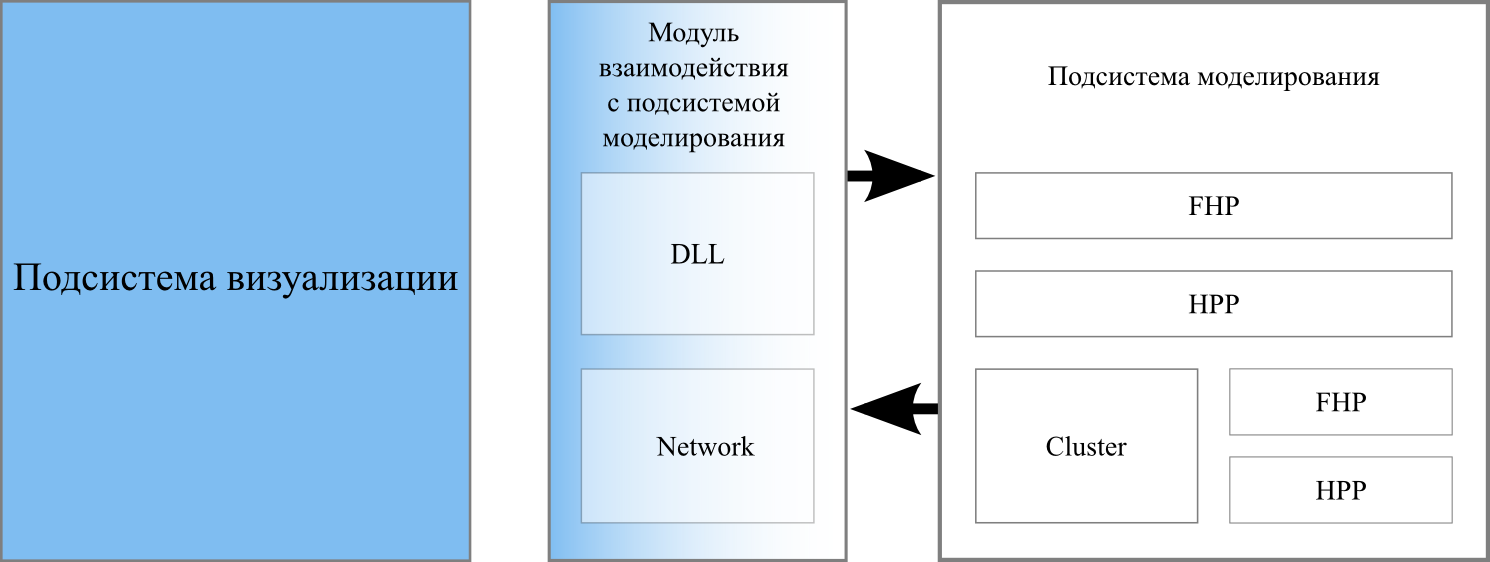
\includegraphics[width=1\linewidth]{architecture-calc}}
        \caption{Взаимодействие с подсистемой моделирования}
        \label{ris:architecture-calc}
    \end{figure}
    
    Для обеспечения коммуникации подсистемы визуализации с подсистемой моделирования был создан интерфейс для добавления поддержки вычислителей.

    В основные функции, решаемые данным модулем, входит запуск процесса моделирования в интерактивном (запуск на счёт фиксированного количества итераций, ожидание завершения моделирования и получение результата) и в пакетном (запуск на счёт с возможностью подключения к вычислителю в любой момент и получения текущего состояния модели) \textit{режимах} и реализация протокола передачи объекта данных с подсистемы моделирования в подсистему визуализации.

    Класс возможных вычислителей, с которыми может взаимодействовать подсистема визуализации, программно ничем не ограничен. Таким образом, в качестве подсистемы моделирования может выступать приложение, запущенное на абсолютно любом устройстве: как процессор или видеокарта локальной машины, так и удалённый кластер, с которым, возможно, требуется общение по уже существующему протоколу (вполне стандартна ситуация, когда доступ к кластеру осуществляется по SSH с необходимостью авторизации).

    Подключение нового вычислителя осуществляется написанием реализации созданного интерфейса. Подробнее о реализации данного модуля написано в приложении~Б. На данный момент реализована поддержка разделяемых библиотек для запуска счёта на локальной машине и в процессе разработки поддержка запуска счёта на удалённой машине, в том числе и для моделирования на кластере.

    %Т.о. система удовлетворяет свойству интероперабельности. <- \textit{надо куда-то красивее вписать}.
\end{subsection}

\begin{subsection}{Модуль поддержки графических библиотек}
    \label{sec:architecture-graphics}
    \begin{figure}[h]
        \center{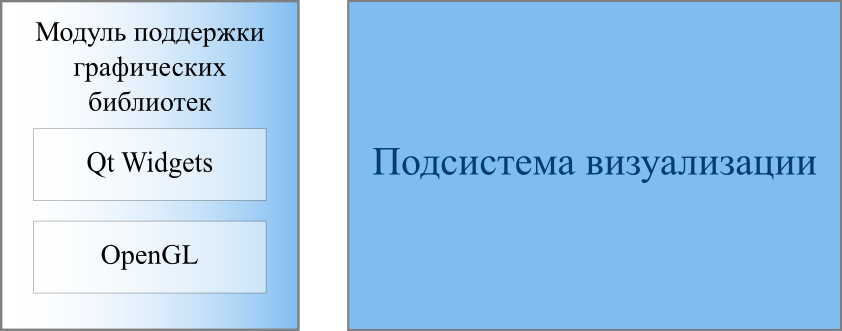
\includegraphics[width=.6\linewidth]{architecture-graphics}}
        \caption{Модуль поддержки графических библиотек}
        \label{ris:architecture-graphics}
    \end{figure}
    
    Поскольку основной задачей инструмента визуализации является создание изображений из объекту данных, то в состав системы так же был включён модуль, отвечающий за поддержку различных графических библиотек. На данный момент существует множество библиотек, как для работы с двухмерной графикой (GTK, Qt, wxWidgets и многие другие), так и с трёхмерной графикой (OpenGL, Direct3D и т.д.). Основной задачей модуля является предоставление общего интерфейса для рисования независимо от того, какая из библиотек используется в данный момент для формирования итогового изображения.

    Модуль поддержки графических библиотек, как и модуль взаимодействия с подсистемой моделирования, включает в себя интерфейс, через реализацию которого осуществляется подключение новой библиотеки. В интерфейс входит рисование графических 2D и 3D примитивов (точки, линии, закрашивание областей), рисование более сложных объектов (различного рода кривые, объединение и пересечение объектов), поддержка прозрачности, если таковая есть в библиотеки. Иными словами, задачей интерфейса является предоставление универсального доступа к возможностям библиотек, скрыв при этом различия при работе с ними для других модулей.

    За счёт введения интерфейса достигается расширяемость, а отсутствие привязанности интерфейса к каким-либо конкретным технологиям делает систему переносимой. Стоит отметить, что некоторые графические библиотеки являются платформозависимыми (например, возможность использовать Direct3D имеется только под операционной системой Microsoft Windows), однако, в целом это не делает систему непереносимой.

    На данный момент используются следующие кроссплатформенные библиотеки:
    \begin{itemize}
        \item Модули QtGUI и QtWidgets из библиотеки Qt.
        \item Библиотека OpenGL для рисования 3D изображений.
    \end{itemize}
\end{subsection}

\begin{subsection}{Модуль поддержки режимов визуализации}
    \label{sec:architecture-render}
    \begin{figure}[h]
        \center{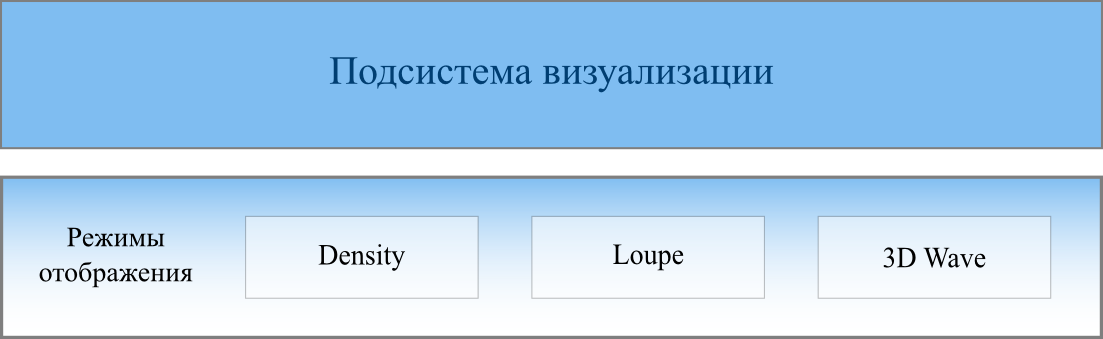
\includegraphics[width=.8\linewidth]{architecture-render}}
        \caption{Модуль поддержки графических библиотек}
        \label{ris:architecture-render}
    \end{figure}
    
    В разделе \ref{sec:requirements-adequacy} одним из требований, предъявляемых к системе, является предоставление исследователю как возможность наблюдать за изменениями отдельных различных характеристик, так и возможность увидеть целостную картину. Данный модуль реализует поддержку различных режимов визуализации и предоставляет возможности для встраивания новых режимов.

    Единственная функция, которую реализует модуль поддержки режимов визуализации, это отображение части или всего объекта данных в двухмерное или трёхмерное изображение. При рисовании изображения данный модуль использует интерфейс, предоставляемый модулем поддержки графических библиотек, а работа с объектом данных модели происходит через модуль взаимодействия с подсистемой моделирования. 

    С помощью интерфейсов данного модуля достигается расширяемость системы: появляется возможность встраивать новые режимы визуализации, при этом не затрагивая обмен данных с вычислительной подсистемой и не внося изменения в существующие форматы данных.

    Добавление поддержки режима визуализации включает в себя реализацию интерфейсов, отвечающих за рисование изображения и за пользовательский интерфейс с настройками режима визуализации. Подробнее о поддержке режимов отображения написано в Приложении В.
    
    На данный момент реализованы:
    \begin{itemize}
        \item Режим среза для изучения профиля волны.
        \item Режим осреднения (статистически-обобщённый).
        \item Режим лупы, позволяющий работать с объектами данных на микроуровне.
        \item 3D режим для получения полноценной картины.
    \end{itemize}
\end{subsection}

\begin{subsection}{Пользовательский интерфейс}
    \label{sec:architecture-ui}
    
    \begin{figure}[h]
        \center{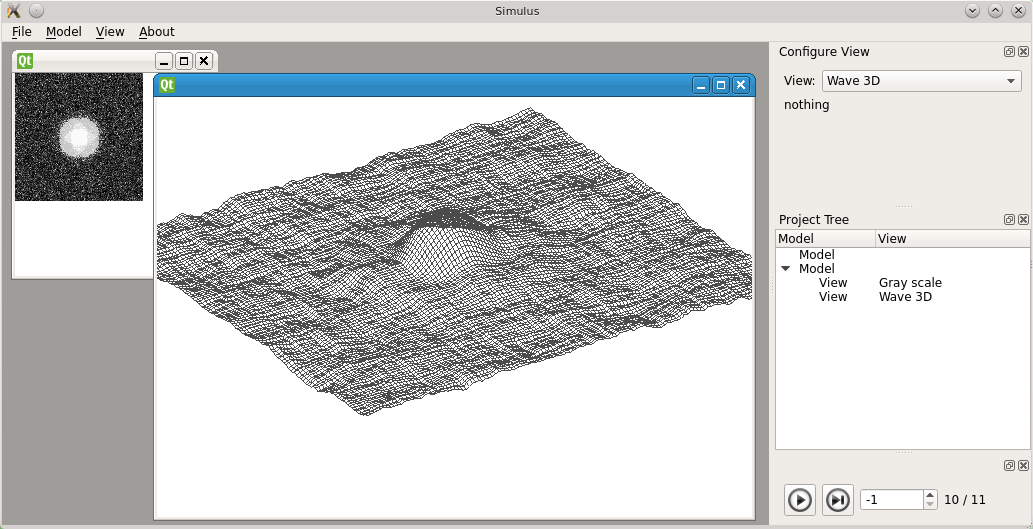
\includegraphics[width=.9\linewidth]{architecture-ui}}
        \caption{Пользовательский интерфейс подсистемы визуализации}
        \label{ris:architecture-ui}
    \end{figure}
    
    Для взаимодействия с пользователем системы был реализован графический интерфейс. Задачей модуля было предоставить пользователю простой, но в тоже время функциональный, удобный, интуитивно-понятный интерфейс. Графический интерфейс направлен на удовлетворение свойству адекватности предметной области: через него пользователь осуществляет работу с проектами и моделями, запуск и наблюдение за процессом моделирования, получение и исследование результатов моделирования, наличие средств для отладки модели.
    
    Пользовательский интерфейс представляем из себя MDI (multiple document interface --- многодокументный интерфейс) окно, внутри которого расположены панели управления, dockable-окна с различными настройками и окна моделей, на которых визуализируются объекты данных.
    Пример запущенного приложения с открытыми окнами модели представлен на рисунке~\ref{ris:architecture-ui}. Пример сценария работы с моделью представлен в Приложении~Г.
        
    \newpage
    . % textit{fix}
\end{subsection}


\section*{Заключение}
\addcontentsline{toc}{section}{Заключение} % Добавляем в содержание раздел без номера

В результате работы были сформулированы требования к подсистеме визуализцаии, разработана архитектура данной подсистемы и построена реализация, выполняющая минимальный набор требуемых функций и включающая следующий набор основных модулей: модуля взаимодействия с подсистемой моделирования, модуля поддержки режимов визуализации, модуля поддержки графических библиотек и пользовательский интерфейс. Спроектирован и реализован протокол, обеспечивающий возможность запуска и управления счётной подсистемы, реализующей КА гидродинамическую модель (НРР), дополненную взвешенными частицами покоя, из подсистемы визуализации на локальной машине.

Реализация подсистемы может быть использована для исследования волновых процессов в средах с разными волновыми характеристиками с помощью клеточно-автоматных моделей газовой динамики. В частности, разработаны режимы визуализации поля скоростей и амплитуд волн в ограниченных пространствах разной конфигурации.

К числу приоритетных направлений дальнейшего развития можно отнести:
\begin{enumerate}
    \item разработку режимов визуализации;
    \item обеспечение возможности взаимодействия со счётными программами, исполняющимися на удалённых машинах, кластерах и ГРИД системах. В первую очередь такая возможность будет реализована для кластера Сибирского Суперкомпьютерного Центра (ССКЦ).
\end{enumerate}





\section*{Приложение А. Сравнение систем визуализации}
\begin{center}
    (Обязательное)
\end{center}
\addcontentsline{toc}{section}{Приложение А. Сравнение систем визуализации}

\begin{table}[h]
        \caption{Соответствие систем визулизации предъявленным требованиям}
        \label{tabular:allsystems}
        \begin{center}
            \begin{tabular}{|r|p{0.4\linewidth}|c|c|c|c|c|c|} \hline
                \textbf{\#} & \textbf{Система}    & \textbf{A$^1$} & \textbf{Р$^2$} & \textbf{И$^3$} & \textbf{П$^4$} & \textbf{Д$^5$} & \textbf{Б$^6$} \\ \hline
               % 1 & Mirek's Celebration & +          & $\mp$      \\ \hline
               % 2 & WinALT              & +          & +          \\ \hline
                
            \end{tabular}
        \end{center}
        \textit{1) А --- Адекватность предметной области \newline
                2) Р --- Расширяемость \newline
                3) И --- Интерактивность \newline
                4) П --- Переносимость \newline
                5) Д --- Дружественность пользовательского интерфейса \newline
                6) Б --- Поддержка больших объёмов данных}
    \end{table}

\section*{Приложение Б. Реализация модуля взаимодействия с подсистемой моделирования}
\begin{center}
    (Рекомендуемое)
\end{center}
\renewcommand{\thesubsection}{\Asbuk{section}.\arabic{subsection}}
\setcounter{section}{2}
\setcounter{subsection}{0}
\addcontentsline{toc}{section}{Приложение Б. Реализация модуля взаимодействия с подсистемой моделирования}

Одной из основных функций системы является коммуникация с подсистемой моделирования. В основном этом передача модели (свойства модели и объект данных) и управляющие команды (запуск, остановка, получение информации о состоянии процесса моделирования и т. п.).

Как было сказано в разделе~\ref{sec:architecture-calc}, добавление поддержки вычислителя возможно за счёт реализации интерфейса, код которого приведён в листинге~\ref{src:calc}.

\begin{lstlisting}[label=src:calc,caption=Интерфейс подключения вычислителя]
class Config : public QObject
{
    Q_OBJECT

    Config(const Config& );
    Config& operator=(const Config& );

protected:

    int current_iteration_id;

    Config();

    void preSerialize  (QDataStream& stream);
    void preDeserialize(QDataStream& stream);

public:

    virtual ~Config();

    virtual int nextIteration();
    virtual int setIteration(int iteration) = 0;
    virtual int getIterationsCount();

    virtual void* getData(void* data_type = NULL) = 0;
    virtual int getDimSize(int dim) const = 0;
    virtual int getDimSizeX() const;
    virtual int getDimSizeY() const;
    virtual int getDimSizeZ() const;

    virtual void serialize  (QDataStream& );
    virtual void deserialize(QDataStream& );
};
\end{lstlisting}

Интерфейс представляет из себя класс с набором виртуальных методов, который можно логически разделить на 3 части:
\begin{enumerate}
    \item управление счётом (запуск, остановка);
    \item работа с объектом данных;
    \item сохранение и загрузка модели.
\end{enumerate}

Б\'oльшая часть виртуальных методов уже имеет простую реализацию и для добавления поддержки нового вычислителя достаточно реализовать всего три метода. За что отвечает каждый из методов и какие из них необходимо реализовывать будем рассмотрено далее.

\subsection{Управление счётом}

% Я пакет и не знаю, как отключить строку с заголовком в listings
\begin{lstlisting}[firstnumber=21,title=~~~~Запуск и остановка процесса моделирования происходит с использованием следующих функций:]
    virtual int nextIteration();
    virtual int setIteration(int iteration) = 0;
    virtual int getIterationsCount();
\end{lstlisting}

Основным является метод \textsf{setIteration(int iteration)} и требует определения при реализации интерфейса. Вызов данного метода означает запуск счёта от последней посчитанной итерации до итерации номер \textsf{iteration}.

Метод \textsf{nextIteration()} запускает счёт на одну итерацию. В реализации по умолчанию он содержит внутри вызов \textsf{setIteration} от номера текущей итерации плюс 1 и позволяет упростить написание и чтение кода.

\textsf{getIterationsCount()} возвращает количество посчитанных итераций.



\subsection{Работа с объектом данных}

\begin{lstlisting}[firstnumber=25,title=Получение объекта данных происходит с использованием следующих функций:]
    virtual void* getData(void* data_type = NULL) = 0;
    virtual int getDimSize(int dim) const = 0;
    virtual int getDimSizeX() const;
    virtual int getDimSizeY() const;
    virtual int getDimSizeZ() const;
\end{lstlisting}

Метод \textsf{getData(void* data\_type)} возвращает часть или весь объект данных. Формат возвращаемого значения зависит от параметра \textsf{data\_type}.

Метод \textsf{getDimSize(int dim)} иммет смысл, когда объект данных является многомерным массивом (в том числе одномерным) и возвращает количество элементов в размерности \textsf{dim}. Методы \textsf{getDimSizeX()}, \textsf{getDimSizeY()} и \textsf{getDimSizeZ()} работают аналогично \textsf{getDimSize(int dim)} для размерности соответственно 0, 1 и 2. Во-первых, они улучшают читаемость кода, во-вторых, в некоторых случаях могут положительно повлиять на производительность.

\subsection{Сохранение и загрузка модели}

\begin{lstlisting}[firstnumber=31]
    virtual void serialize  (QDataStream& );
    virtual void deserialize(QDataStream& );
\end{lstlisting}

Сериализация и десериализация объектов применяется соответственно при сохранении и загрузки проекта. Реализацию данных методов можно оставить пустой, в таком случае проект, в котором используется данная реализация работы с подсистемой вычисления, будет невозможно сохранить и загрузить.



\section*{Приложение В. Реализация модуля поддержки режимов визуализации}
\begin{center}
    (Рекомендуемое)
\end{center}
\setcounter{section}{3}
\setcounter{subsection}{0}
\addcontentsline{toc}{section}{Приложение В. Реализация модуля поддержки режимов визуализации}

Добавление поддержки нового режима визуализации осуществляется реализацией двух интерфейсов, один из которых отвечает за рисования изображения, а другой предоставляет пользовательский интерфейс для конфигурации данного режима.

\subsection{Рисование изображения}

\begin{lstlisting}[label=src:render,caption=Интерфейс добавления поддержки режима визуализации]
class Renderer : public QObject
{
    Q_OBJECT

    Renderer(const Renderer& );
    Renderer& operator=(const Renderer& );

protected:
    Renderer();
    Config *config;
    GraphicBuffer *buffer;

public:
    virtual ~Renderer();

    virtual void setParameters(RendererGUI *);

    virtual void setConfig(Config *_config);
    virtual void setBuffer(GraphicBuffer *_buffer);
    virtual Config* getConfig() const;
    virtual GraphicBuffer* getBuffer() const;

    virtual void prepare() = 0;
    virtual void draw(void *device) = 0;
};
\end{lstlisting}

Класс содержит два свойства: \textsf{Config *config} --- указатель на объект, реализующий взаимодействие с вычислительной подсистемой, и \textsf{GraphicBuffer *buffer} --- указатель на графический буффер, который используется дли рисования. Для обоих свойств определены методы \textsf{set} и \textsf{get}.

Основными методами являются \textsf{void prepare()} и \textsf{void draw(void *device)}. Первый из них вызывается при получении объекта данных от вычислителя, в нём совершаются предварительные вычисления (например, этот метод может использоваться для вычисления осреднённых значений), которые затем понадобятся при рисовании изображения. Второй метод вызывает каждый раз, когда требуется заново отрисовать объект данных. Такое разделение обусловлено тем, что один объект данных требуется перерисовывать каждый раз, когда изменяются параметры режима, однако данные может оказаться достаточным обработать только один раз, т. о. получается выигрыш в производительности. Оба данных метода требуется реализовывать при добавлении поддержки нового режима.

Метод \textsf{setParameters(RendererGUI *)} используется для сопоставления режима визуализации с настройками из пользовательского интерфейса.

\subsection{Графический пользовательский интерфейс}

\begin{lstlisting}[label=src:render-gui,caption=Реализация графического интерфейса для настроек режима визуализации]
class RendererGUI : public QObject
{
    ...

public:
    Q_INVOKABLE RendererGUI(Renderer *_rend);
    virtual ~RendererGUI();

    virtual Renderer* getRenderer() const;

    virtual QString getName() const;
    virtual QWidget* getWidget() const;
};
\end{lstlisting}

В листинге~\ref{src:render-gui} приведён интерфейс для создания графического пользовательского интерфейса с настройками режима визуализации, для краткости в листинге опущены \textsf{private} и \textsf{protected} члены класса как несущественные для ознакомления.

В конструкторе \textsf{RendererGUI(Renderer *\_rend)} создаётся оконный интерфейс, который связывается с объектом \textsf{\_rend}, реализующий режим визуализации.

Метод \textsf{getName()} возвращает название режима визуализации, которое будет использовано в графическом интерфейсе. Метод \textsf{getWidget()} возвращает указатель на окно пользовательского интерфейса.

%\textit{Ссылка на картинку с примером графического интерфейса}


\section*{Приложение Г. Сценарий запуска процесса моделирования}
\addcontentsline{toc}{section}{Приложение Г. Сценарий запуска процесса моделирования}

Работа с моделью начинается с добавления модели в проект --- в систему загружаются все необходимые функции по работе с загружаемой моделью, после чего пользователь имеет возможность управлять созданной моделью. Пример загрузки модели показана на Рис.~\ref{ris:menu_load} и на Рис.~\ref{ris:load_model} --- здесь выбирается динамически-подключаемая библиотека с реализацией модели и указывается файл с начальной конфигурацией.

\begin{figure}[h]
    \center{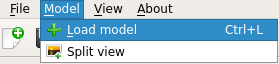
\includegraphics[width=.3\linewidth]{menu_load}}
    \caption{Загрузка модели в проект}
    \label{ris:menu_load}
\end{figure}

\begin{figure}[h]
    \begin{minipage}[h]{0.5\linewidth}
        \center{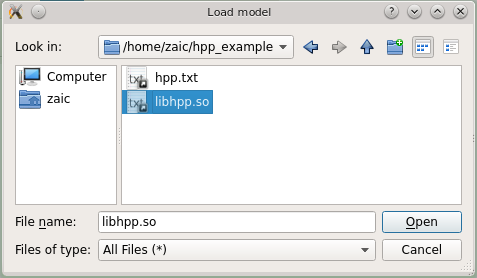
\includegraphics[width=1\linewidth]{load_model_dll}}
    \end{minipage}
    \hfill
    \begin{minipage}[h]{0.5\linewidth}
        \center{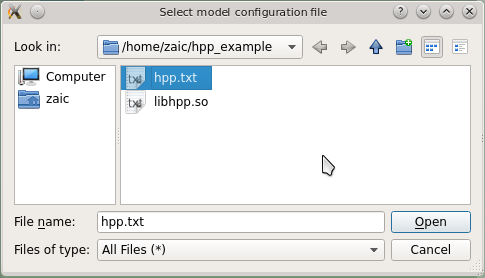
\includegraphics[width=1\linewidth]{load_model_cfg}}
    \end{minipage}
    \caption{Загрузка модели в проект}
    \label{ris:load_model}
\end{figure}

Далее пользователь может запустить модель на счёт с помощью элемента управления, представленного на Рис.~\ref{ris:panel}~в). Может выбирать режимы визуализации и настраивать их параметры (Рис.~\ref{ris:panel}~a)).

\begin{figure}[h]
    \begin{minipage}[h]{0.3\linewidth}
        \center{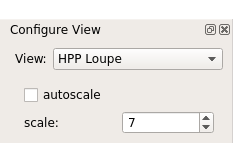
\includegraphics[width=1\linewidth]{panel_config} \\  a)}
    \end{minipage}
    \begin{minipage}[h]{0.3\linewidth}
        \center{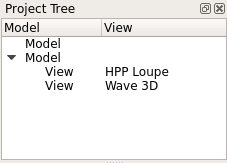
\includegraphics[width=1\linewidth]{panel_models} \\  б)}
    \end{minipage}
    \begin{minipage}[h]{0.3\linewidth}
        \center{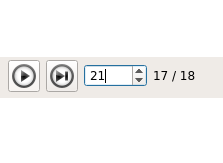
\includegraphics[width=1\linewidth]{panel_calc} \\  в)}
    \end{minipage}
    \caption{Окна работы с моделью}
    \label{ris:panel}
\end{figure}



\renewcommand\refname{Литература}
\addcontentsline{toc}{section}{Литература}
\bibliography{text}

\textit{rename Рекомендуемое}
\textit{предметная область -> проблеманая область}

\end{document}
